\chapter{Statistická analýza výsledků a škálování}
\label{chap:results}

\section{Analýza rozptylu (ANOVA)}
Dekompozice rozptylu validačního BPC ukazuje statistickou signifikanci všech hlavních faktorů i interakcí ($p < 0{,}05$). Celkově model vysvětluje více než 99\,\% rozptylu:
\begin{itemize}
    \item Kapacita modelu: $\eta^2 = 29{,}83\,\%$ ($F = 119{,}21$)
    \item Objem dat: $\eta^2 = 27{,}31\,\%$ ($F = 109{,}14$)
    \item Typ tokenizéru: $\eta^2 = 25{,}16\,\%$ ($F = 50{,}27$)
    \item Interakce Model $\times$ Tokenizer: $\eta^2 = 9{,}50\,\%$
    \item Interakce Data $\times$ Tokenizer: $\eta^2 = 7{,}45\,\%$
\end{itemize}

\section{Empirické škálovací křivky}
Nelineární regrese odhadla parametry Kaplanova zákona na hodnoty:
\begin{equation}
    \text{BPC}(N, D) = 0{,}555 + \frac{77{,}05}{N^{0{,}462}} + \frac{93{,}78}{D^{0{,}390}}
\end{equation}
s odhadem ireducibilní entropie $E \approx 0{,}555$ bitů na znak.

\begin{figure}[htbp]
    \centering
    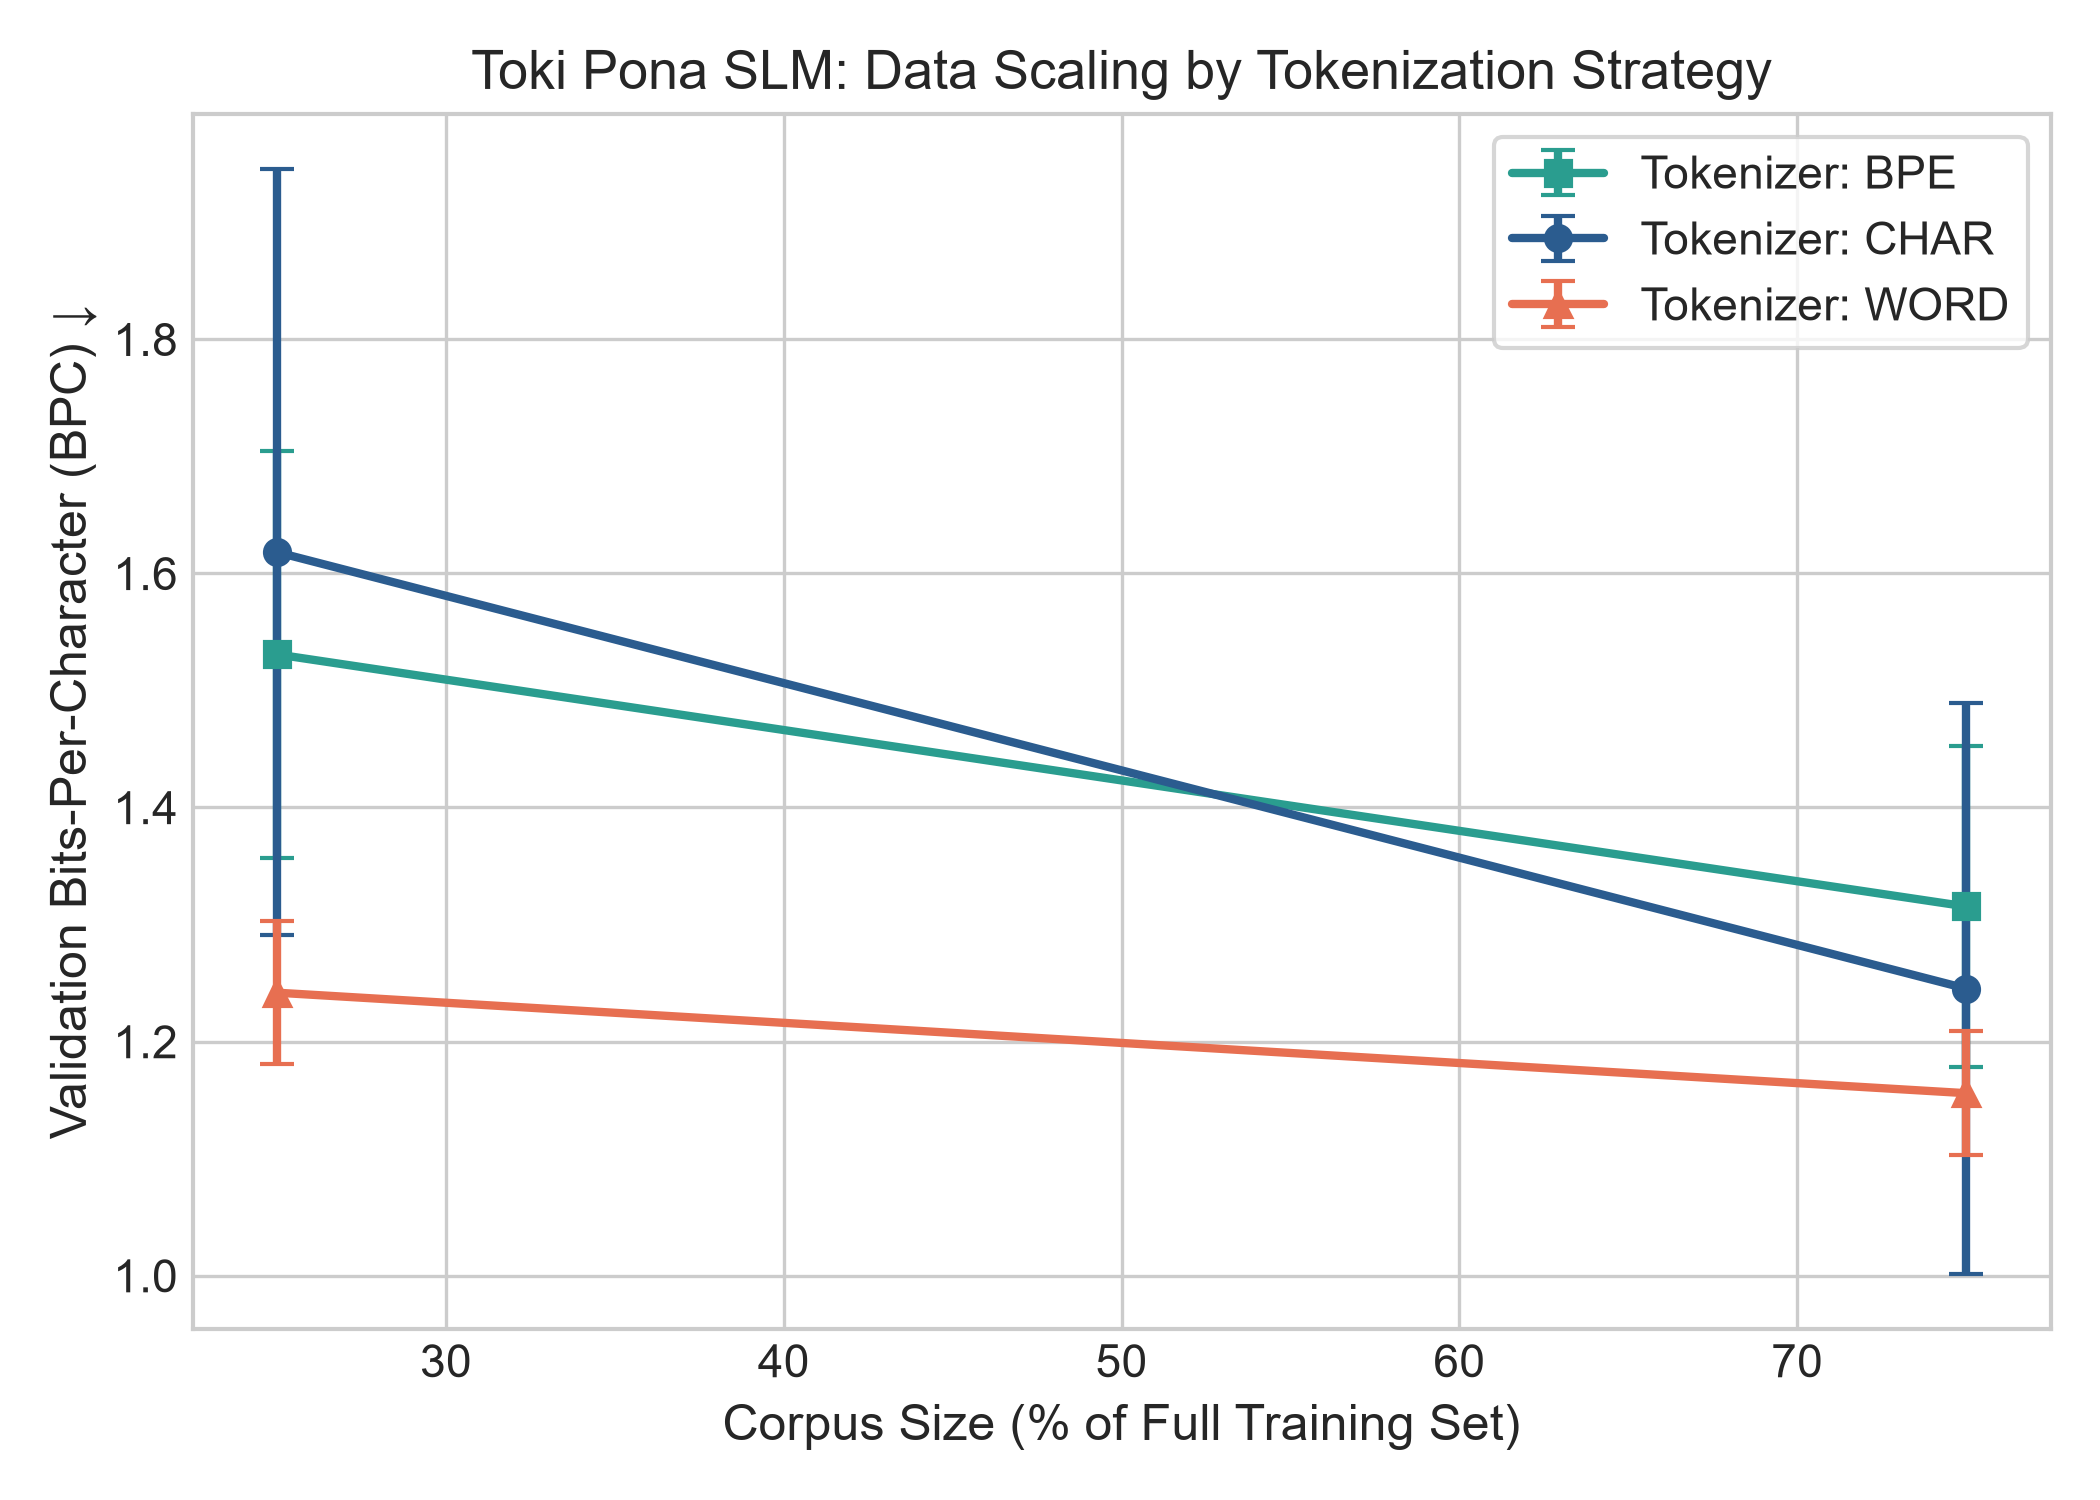
\includegraphics[width=0.8\textwidth]{figures/scaling_data_bpc.png}
    \caption{Závislost Bits-Per-Character na objemu trénovacích dat podle tokenizéru.}
    \label{fig:scaling_data}
\end{figure}

\begin{figure}[htbp]
    \centering
    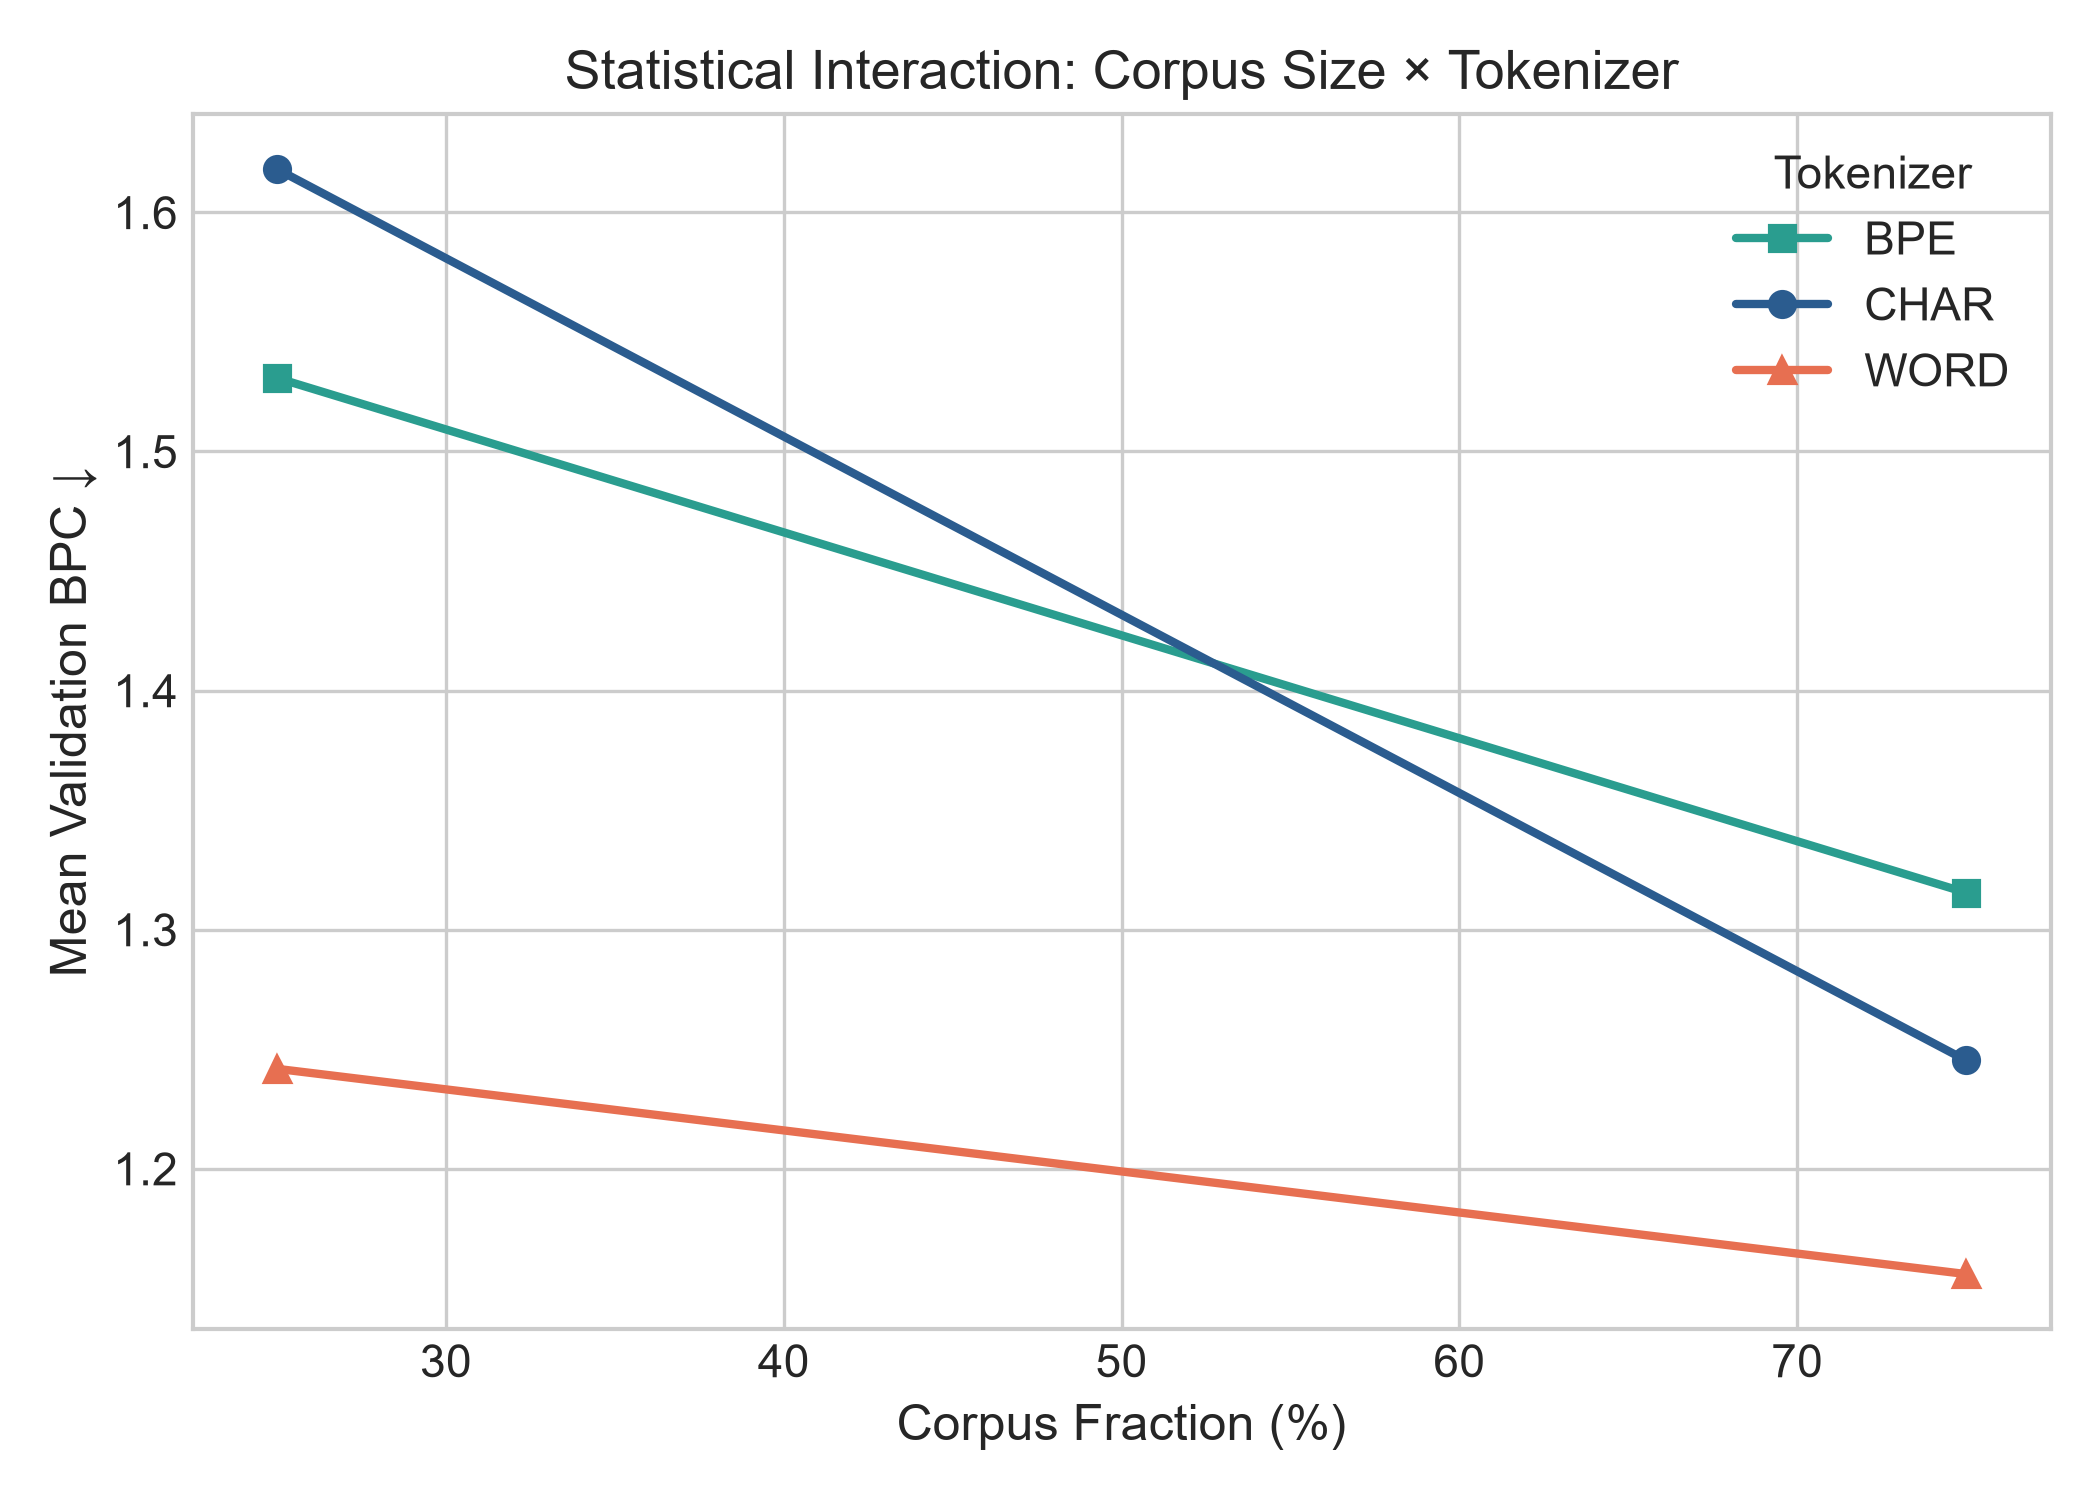
\includegraphics[width=0.8\textwidth]{figures/interaction_effects.png}
    \caption{Interakční graf mezi velikostí korpusu a typem tokenizéru.}
    \label{fig:interaction}
\end{figure}
